\documentclass[UTF8,fontset=fandol,11pt,a4paper]{ctexart}
\usepackage[a4paper,margin=1.75cm,headheight=15pt]{geometry}
\usepackage{amsmath,amssymb,mathtools}
\usepackage{booktabs,longtable,tabularx,array,multirow}
\usepackage{enumitem}
\usepackage[most]{tcolorbox}
\usepackage{tikz}
\usetikzlibrary{arrows.meta,positioning,fit,calc,matrix}
\usepackage{xcolor}
\usepackage{fancyhdr}
\usepackage{hyperref}
\usepackage{microtype}
\usepackage{lastpage}

\newcolumntype{Y}{>{\raggedright\arraybackslash}X}
\newcolumntype{L}[1]{>{\raggedright\arraybackslash}p{#1}}
\newcolumntype{C}[1]{>{\centering\arraybackslash}p{#1}}
\setlength{\parindent}{2em}
\setlength{\parskip}{0.34em}
\setlength{\emergencystretch}{3em}
\renewcommand{\arraystretch}{1.22}
\setlength{\tabcolsep}{3pt}
\setlist[itemize]{itemsep=0.18em,topsep=0.35em,leftmargin=2em}
\setlist[enumerate]{itemsep=0.18em,topsep=0.35em,leftmargin=2em}

\definecolor{deep}{RGB}{38,58,72}
\definecolor{soft}{RGB}{244,247,248}
\definecolor{accent}{RGB}{116,72,46}
\definecolor{greenish}{RGB}{52,91,74}
\definecolor{warnc}{RGB}{136,61,58}
\definecolor{purple}{RGB}{84,72,112}
\definecolor{rulegray}{RGB}{110,116,120}

\hypersetup{
  colorlinks=true,
  linkcolor=deep,
  urlcolor=accent,
  pdftitle={CO-03 CPU 数据通路与控制}
}

\pagestyle{fancy}
\fancyhf{}
\lhead{\small\color{deep}\textbf{408 · 计算机组成原理 CO-03}}
\rhead{\small\color{deep}数据通路 · 控制 · 提交}
\cfoot{\small 第 \thepage\ 页 / 共 \pageref{LastPage} 页}
\renewcommand{\headrulewidth}{0.4pt}

\newtcolorbox{corebox}[1]{breakable,colback=soft,colframe=deep,title=\textbf{#1},boxrule=0.8pt,arc=2mm}
\newtcolorbox{methodbox}[1]{breakable,colback=white,colframe=greenish,title=\textbf{#1},boxrule=0.7pt,arc=1.5mm}
\newtcolorbox{warnbox}[1]{breakable,colback=white,colframe=warnc,title=\textbf{#1},boxrule=0.7pt,arc=1.5mm}
\newtcolorbox{examplebox}[1]{breakable,colback=white,colframe=purple,title=\textbf{#1},boxrule=0.7pt,arc=1.5mm}
\newcommand{\kw}[1]{\textbf{\color{deep}#1}}
\newcommand{\code}[1]{\texttt{#1}}

\tikzset{
  co/.style={draw=deep,rounded corners=1.5mm,text width=2.6cm,minimum height=0.95cm,align=center,fill=soft,font=\small,inner sep=3pt},
  state/.style={co,double,double distance=1.2pt,fill=white},
  abstract/.style={co,fill=black!8},
  flow/.style={-{Latex[length=2mm]},thick,draw=deep},
  ref/.style={-{Latex[length=2mm]},dashed,draw=rulegray},
  fast/.style={-{Latex[length=2mm]},dotted,thick,draw=purple}
}

\title{\vspace{-1.1cm}\textbf{CPU 数据通路与控制}\\[0.4em]
\large 从 ISA 状态差到可计时、可验证的精确提交}
\author{408 · 计算机组成原理 Topic CO-03}
\date{}

\begin{document}
\maketitle

\begin{corebox}{母问题：一条指令承诺的状态变化，怎样由有限硬件真正发生？}
ISA 只规定软件应当观察到什么变化；数据通路和控制器必须决定这些变化由哪些值、部件、路径和时钟边界实现。本册的生成链是
\[
\boxed{
\text{ISA State Delta}
\to\text{Required Values}
\to\text{Producer--Consumer Graph}
\to\text{Datapath}
\to\text{Resource Schedule}
\to\text{Control Word}
\to\text{Clock Boundary}
\to\text{Precise Commit}
}
\]
箭头表示设计依赖：后一步必须能够实现前一步，而不能反过来用某张教材通路图篡改指令语义。
\end{corebox}

\begin{methodbox}{本册定位与 Owner 边界}
\begin{itemize}
  \item \kw{Owns：}架构状态与微架构状态边界；状态差到通路的生成；微操作可行性；单周期/多周期调度；控制信号生成；关键路径与精确提交。
  \item \kw{Uses：}CO-02 的 ISA 指令语义与地址形成；CO-05 的抽象存储接口。
  \item \kw{Stops：}多条指令的时间重叠交给 CO-04；Cache、TLB 和 Page Walk 交给 CO-06/07；中断进入 OS 后的软件动作交给跨科 Bridge。
\end{itemize}
\end{methodbox}

\tableofcontents
\newpage

\section{为什么“取指、译码、执行”还不是模型}

阶段名只能描述大致顺序，不能回答以下问题：
\begin{itemize}
  \item 哪一个值由谁产生，下一步由谁消费？
  \item 两个动作能否同拍发生，还是争用同一条总线或 ALU？
  \item 一个中间结果已经算出，是否已经改变软件可见状态？
  \item 控制器为何打开这个写使能，又为何必须关闭另一个写使能？
\end{itemize}

真正可生成通路的起点不是阶段名，而是指令的\kw{状态差}。设软件可见架构状态为
\[
A=(PC,R,M,F,\ldots),
\]
其中 $R$ 表示架构寄存器集合，$M$ 表示内存可见状态，$F$ 表示架构标志或条件状态。一条指令定义状态转移
\[
A_{t+1}=\mathcal{I}(A_t).
\]

例如抽象指令
\[
\code{ADD rd, rs1, rs2}
\]
承诺的主要状态差是
\[
R'[rd]=R[rs1]+R[rs2],\qquad PC'=PC+L,
\]
其余架构状态保持不变。这里的 $L$ 是该 ISA 规定的顺序取指步长，不应无条件写死为 4。

\begin{warnbox}{第一条禁推关系}
教材图中出现 PC 加法器、MAR、MDR 或某个固定节拍，不表示 ISA 要求所有实现都拥有这些具体部件。ISA Own ``必须发生什么''；本册 Own ``一种实现怎样保证它发生''。
\end{warnbox}

\section{两类状态：软件契约与内部实现}

\subsection{架构状态}

架构状态（architectural state）是 ISA 允许软件观察或依赖的状态，例如通用寄存器、PC、架构标志、可见内存效果和规定的控制寄存器。处理器完成一条指令后，必须给出符合 ISA 的下一状态。

\subsection{微架构状态}

微架构状态（microarchitectural state）服务于实现，例如 IR、MAR、MDR、临时寄存器、控制状态寄存器、流水寄存器和 Cache 内部元数据。它们可以随实现不同而变化，但不能让软件看到违反 ISA 的结果。

\[
\boxed{
\text{internal states may differ}
\quad\land\quad
\text{architectural trace must remain ISA-equivalent}
}
\]

\begin{examplebox}{同一条 ADD 的两种实现}
实现甲在一个长周期内完成寄存器读取、加法和写回；实现乙先把两个源值锁存到临时寄存器，下一拍相加，再下一拍写回。两者内部状态轨迹不同，但只要提交后的 $R[rd]$、PC 和异常语义一致，就实现了同一条 ISA 指令。
\end{examplebox}

\subsection{可访问性不能脱离 ISA 断言}

旧笔记把寄存器固定分为“用户可见、部分可见、系统可见、完全不可见”四级，这个观察方向有价值，但具体归类依赖 ISA：
\begin{itemize}
  \item PC、标志寄存器能否显式读写，取决于指令集；
  \item 页表基址、Cache 管理和 MMU 控制可能存在特权接口；
  \item PCB 指针通常是 OS 软件状态，不是必然存在的 CPU 专用寄存器；
  \item “对普通用户透明”不等于“对 OS 或固件完全不可见”。
\end{itemize}
稳定判据不是背清单，而是问：\kw{当前 ISA 是否提供了读取、写入、配置或间接影响该状态的合法操作？}

\section{从状态差生成值依赖图}

对任意指令，先列四类量：
\begin{enumerate}
  \item \kw{Read Set：}完成语义必须读取哪些架构值？
  \item \kw{Derived Values：}中间必须产生哪些值？
  \item \kw{Write Set：}哪些架构位置允许改变？
  \item \kw{Next PC / Exception：}正常路径和异常路径怎样结束？
\end{enumerate}

\subsection{四条母指令}

\begin{center}
\small
\begin{tabularx}{\linewidth}{L{2.1cm}YYYY}
\toprule
指令族 & Read Set & Derived Values & Write Set & 关键禁写 \\
\midrule
ADD & 两个源寄存器、PC & 算术结果、顺序 PC & 目标寄存器、PC & 内存不得被写 \\
LOAD & base、立即数、PC & 有效地址、返回数据、扩展值 & 目标寄存器、PC & 内存内容不得被改 \\
STORE & base、data、立即数、PC & 有效地址、写数据、byte mask & 指定内存位置、PC & 通用目标寄存器不得误写 \\
BRANCH & 源值、PC、偏移 & 条件、目标 PC、顺序 PC & PC，可能还有架构约定状态 & 错路指令不得提交 \\
\bottomrule
\end{tabularx}
\end{center}

\subsection{LOAD 的生产者--消费者图}

抽象 LOAD 可写成：
\[
EA=R[base]+\operatorname{ext}(imm),
\qquad
D=M[EA],
\qquad
R'[rd]=\operatorname{ext}_{width}(D).
\]

\begin{center}
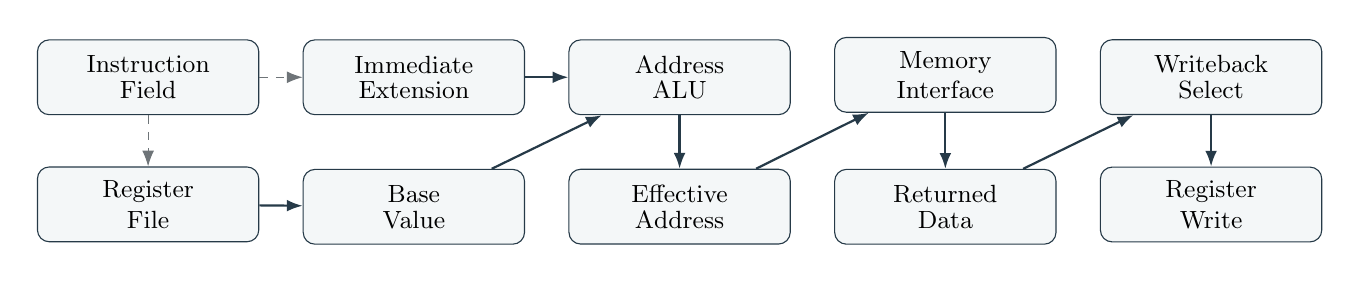
\begin{tikzpicture}[node distance=0.65cm and 0.8cm]
\matrix[matrix of nodes,column sep=0.55cm,row sep=0.65cm,nodes={co},ampersand replacement=\&] (m) {
\shortstack{Instruction\\Field} \& \shortstack{Immediate\\Extension} \& \shortstack{Address\\ALU} \& \shortstack{Memory\\Interface} \& \shortstack{Writeback\\Select} \\
\shortstack{Register\\File} \& \shortstack{Base\\Value} \& \shortstack{Effective\\Address} \& \shortstack{Returned\\Data} \& \shortstack{Register\\Write} \\
};
\draw[ref] (m-1-1) -- (m-1-2);
\draw[ref] (m-1-1) -- (m-2-1);
\draw[flow] (m-2-1) -- (m-2-2);
\draw[flow] (m-1-2) -- (m-1-3);
\draw[flow] (m-2-2) -- (m-1-3);
\draw[flow] (m-1-3) -- (m-2-3);
\draw[flow] (m-2-3) -- (m-1-4);
\draw[flow] (m-1-4) -- (m-2-4);
\draw[flow] (m-2-4) -- (m-1-5);
\draw[flow] (m-1-5) -- (m-2-5);
\end{tikzpicture}
\end{center}

这张图的箭头表示数据依赖，不先承诺在哪一拍执行。先得到依赖图，再选择资源和调度，能够避免“照着已有图猜控制信号”。

\section{数据通路的最小构件}

\begin{center}
\small
\begin{tabularx}{\linewidth}{L{2.4cm}YYL{3.4cm}}
\toprule
构件 & 它提供什么能力 & 它不自动保证什么 & 常见约束 \\
\midrule
状态元件 & 跨时钟边界保存值 & 保存的值一定属于架构状态 & setup/hold、写使能、复位 \\
组合逻辑 & 在当前输入上计算函数 & 结果已经提交 & 传播延迟、扇出、关键路径 \\
MUX & 从候选来源中选一路 & 被选来源语义正确 & 选择信号、输入数、额外延迟 \\
寄存器堆 & 按编号读写架构寄存器 & 所有实现都同拍两读一写 & 端口数、读写同址语义 \\
存储接口 & 发请求并收发数据 & 请求一定本拍返回 & latency、ready/valid、异常 \\
总线 & 多部件共享传输媒介 & 多个源可同时驱动 & 仲裁、唯一驱动、带宽 \\
控制器 & 产生使能、选择和下一阶段 & 数据值本身正确 & 输入条件完整、无非法组合 \\
\bottomrule
\end{tabularx}
\end{center}

\begin{corebox}{数据通路和控制通路的分工}
\[
\boxed{
\text{Datapath: what values can move and transform}
\qquad
\text{Control: which legal movement happens now}
}
\]
数据通路提供可能性集合；控制器按指令、阶段和条件选出当前合法转移。
\end{corebox}

\section{微操作：把依赖图调度到时钟边界}

微操作是在一个受控阶段内发生的寄存器传送或组合变换。例如单总线教学机中：
\begin{align*}
R_1 &\to Y,\\
Y+R_2 &\to Z,\\
Z &\to R_3.
\end{align*}

能否同拍执行，不由语句长短决定，而要同时通过四道门：
\begin{enumerate}
  \item \kw{Dependency Gate：}所有输入在本拍开始或组合路径要求的时刻已经可用；
  \item \kw{Resource Gate：}总线、端口、ALU、存储口没有互斥占用；
  \item \kw{Timing Gate：}最长组合路径满足时钟约束；
  \item \kw{Commit Gate：}写使能不会产生 ISA 不允许的副作用。
\end{enumerate}

对同步电路，一条基本时序约束可写为
\[
T_{clk}\ge T_{cq}+T_{comb,max}+T_{setup}+T_{skew}.
\]
题目若采用简化模型，可以省略某些项，但必须先声明成本口径。

\begin{warnbox}{单总线规则}
同一时刻通常只允许一个源驱动总线；多个目标可以锁存同一个总线值。两条箭头画得下，不代表两个不同源能够同时输出。
\end{warnbox}

\section{单周期与多周期：同一依赖图的两种调度}

\subsection{单周期实现}

单周期处理器把一条指令的完整依赖链放进一个长组合周期。其 CPI 通常按教学模型取 1，但时钟周期必须覆盖最慢合法路径。
\[
T_{clk}^{single}\ge\max_{i\in\text{instructions}}T_{path}(i).
\]

它的核心代价不是“控制简单”四个字，而是：
\begin{itemize}
  \item 短指令也被最长指令拖住；
  \item 同一拍重复使用某资源时，必须复制资源、增加端口或改变抽象；
  \item 组合路径越长，频率越受限。
\end{itemize}

\subsection{多周期实现}

多周期处理器在阶段边界加入临时状态，把依赖图切成多个较短周期，并允许不同阶段复用同一资源：
\[
T_{instr}(i)=C_iT_{clk}^{multi}.
\]
其中 $C_i$ 是指令 $i$ 的周期数。周期数变大并不自动变慢，因为 $T_{clk}^{multi}$ 通常更短。

\subsection{公平比较}

\[
\boxed{T_{CPU}=IC\times CPI\times T_{clk}}
\]
比较实现时必须使用同一程序、同一指令统计口径，并同时考虑指令混合、周期时间和 CPI。单独比较“CPI=1”或“频率更高”都不足以判快慢。

\begin{center}
\small
\begin{tabularx}{\linewidth}{L{2.5cm}YY}
\toprule
维度 & 单周期 & 多周期 \\
\midrule
调度单位 & 一条指令一个长周期 & 一条指令多个短阶段 \\
中间状态 & 尽量不跨拍保存 & 用 IR/MDR/临时寄存器保存 \\
资源策略 & 复制或增加端口以消除同拍冲突 & 分时复用资源 \\
控制输入 & 主要是指令与条件 & 指令、当前阶段与条件 \\
主要风险 & 最长路径拖慢全部指令 & 状态机、暂存与控制更复杂 \\
性能判断 & $1\times T_{clk}^{single}$ & $C_i\times T_{clk}^{multi}$ \\
\bottomrule
\end{tabularx}
\end{center}

\begin{warnbox}{旧笔记中的过度结论}
“单周期必须采用哈佛结构”“寄存器堆读端口永远无需使能”“LOAD 必然是最长路径”都只能在给定教学数据通路和存储时序下成立。稳定正文保留资源冲突与关键路径判据，不把某个实现选择升级为体系结构定律。
\end{warnbox}

\section{控制器：把条件映射为控制字与下一阶段}

控制器解决的统一问题是
\[
\boxed{
(instruction,phase,condition)
\longmapsto
(control\ word,next\ phase)
}
\]

控制字至少会包含三类决策：
\begin{itemize}
  \item \kw{Enable：}哪些状态元件允许写入；
  \item \kw{Select：}MUX、ALU 和数据来源选哪一路；
  \item \kw{Command：}存储读写、异常请求、阶段推进等动作。
\end{itemize}

\subsection{硬布线控制}

硬布线控制用组合/时序逻辑直接实现上述映射。它没有“不要经过任何状态”这一要求：多周期硬布线控制通常仍然是一个 FSM。其优势是避免逐条读取控制存储的开销，代价是复杂逻辑的设计、验证和修改成本。

\subsection{微程序控制}

微程序控制把控制字和下一微地址组织为微指令，存放在控制存储器中。机器指令触发某段微程序入口，微顺序器按条件选择后继微指令。

\begin{center}
\small
\begin{tabularx}{\linewidth}{L{2.2cm}YYL{3.5cm}}
\toprule
维度 & 硬布线 & 微程序 & 稳定判据 \\
\midrule
映射载体 & 逻辑网络/FSM & 控制存储+微顺序器 & 都必须生成同一合法控制效果 \\
速度来源 & 避免控存读取链 & 结构规整、便于复杂序列 & 具体快慢取决于实现与技术 \\
修改成本 & 逻辑重设计成本高 & 修改微码相对集中 & 不等于 ISA 可随意修改 \\
常见误区 & “只属于 RISC” & “只属于 CISC” & 现代实现可以混合 \\
\bottomrule
\end{tabularx}
\end{center}

RISC/CISC 描述 ISA 设计取向，硬布线/微程序描述控制实现。两组概念相关，但不存在一一绑定。

\section{提交：写使能才是架构状态变化的闸门}

一个值在 ALU 输出端稳定，只说明它\kw{已经产生}；被后级路径选中，只说明它\kw{可以到达}；只有在合法时钟边界打开正确状态元件的写使能，它才\kw{提交}为新状态。

\[
\boxed{
\text{Produced}
\neq
\text{Available at Destination}
\neq
\text{Architecturally Committed}
}
\]

这一区分提供一个强校验：对照指令 Write Set，检查所有可能写口。
\begin{itemize}
  \item 应写的位置是否真的打开？
  \item 不应写的位置是否全部关闭？
  \item 若发生异常，故障指令是否留下了禁止的部分副作用？
  \item PC 的正常值、分支值和异常入口是否由互斥条件选择？
\end{itemize}

精确异常的跨科接口只保留最小要求：异常前较老的架构效果已经成立；故障指令及更年轻指令的禁止副作用没有提交。具体 OS handler 不属于本册。

\section{概念边界：相似名词为什么会误导通路题}

\begingroup
\footnotesize
\renewcommand{\arraystretch}{1.28}
\begin{longtable}{L{2.25cm}C{0.45cm}L{2.25cm}L{6.0cm}L{3.0cm}}
\toprule
概念 A & & 概念 B & 真正区别与题目信号 & 混淆后果 \\
\midrule
\endfirsthead
\toprule
概念 A & & 概念 B & 真正区别与题目信号 & 混淆后果 \\
\midrule
\endhead
架构状态 & $\neq$ & 微架构状态 & 软件契约可依赖前者；IR/MDR 等通常只服务实现。问“不同实现能否不同”时先分层。 & 把教学寄存器误写成 ISA 必需部件。 \\
\addlinespace
ISA 语义 & $\neq$ & 数据通路 & 前者规定结果，后者提供实现路径。给指令定义时先写状态差。 & 用某张通路图反向篡改指令语义。 \\
\addlinespace
数据通路 & $\neq$ & 控制器 & 前者定义可能的数据移动，后者选择此刻允许的移动。 & 只连线不检查写使能和冲突。 \\
\addlinespace
组合结果产生 & $\neq$ & 状态提交 & 前者是线路值稳定，后者需要合法写入状态元件。 & 认为 ALU 算完就等于指令完成。 \\
\addlinespace
指令周期 & $\neq$ & 时钟周期 & 一条指令可跨多个时钟周期；题目给“周期”时要确认量纲。 & CPI、节拍和总时间混算。 \\
\addlinespace
微操作 & $\neq$ & 微指令 & 微操作是数据动作；微指令是编码若干控制信号的控制存储字。 & 把动作序列与编码载体混为一谈。 \\
\addlinespace
内部 CPU 总线 & $\neq$ & 系统总线 & 前者连接处理器内部部件，后者组织芯片/设备事务；模型和仲裁范围不同。 & 把单总线微操作规则套到外部总线。 \\
\addlinespace
硬布线/微程序 & $\neq$ & RISC/CISC & 前一组是实现机制，后一组是 ISA 设计取向。 & 形成“一一对应”的错误选择题口诀。 \\
\bottomrule
\end{longtable}
\endgroup

\section{贯穿母例：在单总线教学机上实现 LOAD}

设教学机满足以下明确假设：
\begin{itemize}
  \item 字节编址，顺序 PC 步长为 $L$；
  \item CPU 内部只有一条总线，同拍唯一源驱动；
  \item ALU 的一个输入经 $Y$ 暂存，输出经 $Z$ 暂存；
  \item MAR/MDR 与存储接口交互；
  \item 存储读完成由题设时序保证或显式等待信号决定。
\end{itemize}

目标指令为
\[
\code{LOAD rd, imm(rs1)}.
\]

\subsection{先写语义，不先写节拍}
\begin{align*}
EA&=R[rs1]+\operatorname{sext}(imm),\\
D&=M[EA],\\
R'[rd]&=\operatorname{extend}(D),\\
PC'&=PC+L.
\end{align*}

\subsection{再按资源约束调度}

一种合法但非唯一的调度是：
\begin{center}
\small
\begin{tabularx}{\linewidth}{C{1.1cm}L{4.4cm}YY}
\toprule
阶段 & 微操作 & 生产/消费 & 校验 \\
\midrule
$T_1$ & $PC\to MAR,\ PC\to Y$ & 产生取指地址和顺序 PC 输入 & 同一总线源 PC，可多目标锁存 \\
$T_2$ & $M[MAR]\to MDR,\ Y+L\to Z$ & 存储返回指令；ALU 产生下一 PC & 仅在存储与 ALU 可并行假设下同拍 \\
$T_3$ & $Z\to PC$ & 提交顺序 PC & PC 写使能打开 \\
$T_4$ & $MDR\to IR$ & 当前指令进入译码状态 & 不改变通用寄存器 \\
$T_5$ & $R[rs1]\to Y$ & 锁存 base & 寄存器编号来自指令字段 \\
$T_6$ & $Y+\operatorname{sext}(imm)\to Z$ & 产生 EA & 扩展规则来自 ISA \\
$T_7$ & $Z\to MAR$ & 发出数据地址 & 仍未得到 load 数据 \\
$T_8$ & $M[MAR]\to MDR$ & 数据返回 & 若存储未 ready，必须等待 \\
$T_9$ & $MDR\to R[rd]$ & 提交目标寄存器 & MemWrite 必须关闭 \\
\bottomrule
\end{tabularx}
\end{center}

\begin{warnbox}{母例故意暴露的错误路径}
若在 $T_6$ 就打开目标寄存器写使能，写入的是有效地址而非加载数据；若在 $T_8$ 打开内存写信号，则 LOAD 被错误实现成 STORE。两种错误都能通过“Write Set 反查”提前发现。
\end{warnbox}

固定九拍不是知识本体。换成双总线、多端口寄存器堆、独立 PC 加法器或不同存储握手后，调度会改变；状态差、依赖和提交边界不变。

\section{怎样为新指令扩展数据通路}

题目要求“加入某条指令”时，按以下顺序工作：
\begin{enumerate}
  \item 写该指令的 Read Set、Derived Values、Write Set 和 Next PC；
  \item 将每个中间值标成“生产者 $\to$ 消费者”；
  \item 在现有通路上寻找路径，缺路才新增连线、MUX 或功能部件；
  \item 检查端口和资源冲突，决定是否新增阶段或复制资源；
  \item 补充控制信号真值和控制器状态转移；
  \item 重新计算关键路径或新 CPI；
  \item 用 Write Set 和异常路径验证没有多余副作用。
\end{enumerate}

\begin{methodbox}{最小硬件原则}
“支持新指令”不等于先加一个新部件。若现有 ALU、MUX 和暂存寄存器能通过新的调度完成语义，新增控制状态可能比复制硬件更合理；若性能约束不允许多拍，再讨论复制资源。先证明缺什么，再加什么。
\end{methodbox}

\section{性能：从路径和资源生成数字}

\subsection{关键路径}

关键路径不是“部件延迟全部相加”。只有同一周期内、沿真实依赖串联的组合部件才累加；互相并行的路径取最大值。
\[
T_{comb,max}=\max_{p\in\text{legal paths}}\sum_{u\in p}T_u.
\]

\subsection{资源复制与复用}

\begin{center}
\small
\begin{tabularx}{\linewidth}{L{3.0cm}YY}
\toprule
设计动作 & 获得的能力 & 支付的代价 \\
\midrule
增加独立 PC 加法器 & PC 更新可与主 ALU 工作并行 & 面积、功耗、布线 \\
增加寄存器堆端口 & 同拍读取/写入更多值 & 阵列面积与访问延迟 \\
加入更多 MUX 输入 & 复用现有功能部件 & 选择控制与关键路径变长 \\
加入临时寄存器 & 跨拍保存中间值、缩短周期 & 状态和控制阶段增加 \\
复制存储端口 & 消除取指/数据访问冲突 & 存储结构复杂度和成本 \\
\bottomrule
\end{tabularx}
\end{center}

\subsection{题目成本模型}

遇到性能题先写：
\[
\text{what overlaps?}
\quad
\text{what serializes?}
\quad
\text{what is the unit?}
\]
再计算时钟周期、每类指令 CPI、指令混合和总执行时间。若题目没有给 setup、skew 或控制延迟，只能按题设简化，不能暗中加入另一套口径。

\section{做题控制协议}

\begin{corebox}{CO-03 七步协议}
\begin{enumerate}
  \item \kw{Delta：}写指令前后允许变化的架构状态；
  \item \kw{Values：}列 Read Set、Derived Values、Write Set；
  \item \kw{Graph：}标出每个值的生产者和消费者；
  \item \kw{Path：}沿现有部件连可行路径，选择点才放 MUX；
  \item \kw{Schedule：}按依赖、资源、时序和提交四道门拆拍；
  \item \kw{Control：}为每拍写唯一驱动、锁存目标、选择信号和条件；
  \item \kw{Verify：}用 ISA Write Set、关键路径和异常边界做独立反查。
\end{enumerate}
\end{corebox}

\subsection{题目信号与第一动作}

\begin{center}
\small
\begin{tabularx}{\linewidth}{L{4.1cm}Y}
\toprule
题目信号 & 第一动作 \\
\midrule
“补全数据通路/支持新指令” & 写 before/after 状态差，不先画线 \\
“哪些微操作可并行” & 列源、目标、依赖和共享资源 \\
“求控制信号” & 先写当前拍的数据动作，再映射 Enable/Select/Command \\
“单周期与多周期比较” & 写 $IC\times CPI\times T_{clk}$，统一成本口径 \\
“关键路径” & 只沿同一周期真实串联路径求和，再取最大 \\
“发生异常/中断” & 先查哪些架构写口尚未或不得提交 \\
\bottomrule
\end{tabularx}
\end{center}

\section{高频失效模式}

\begin{enumerate}
  \item \kw{从图开始：}记得部件，却不知道为什么需要它。修复：先写 State Delta。
  \item \kw{把箭头当并行：}忽略总线、端口或 ALU 冲突。修复：逐拍列资源占用。
  \item \kw{把产生当提交：}ALU 输出有值就认为寄存器已更新。修复：追踪写使能和时钟边界。
  \item \kw{把实现当 ISA：}认为 MAR/MDR、九节拍或固定 PC 步长普遍存在。修复：给所有实现细节加前提。
  \item \kw{只比 CPI：}宣称单周期 CPI 低所以更快。修复：比较完整 CPU time。
  \item \kw{RISC/CISC 口诀化：}把 RISC 与硬布线、CISC 与微程序绝对绑定。修复：分开 ISA 与实现两条轴。
  \item \kw{越过 Stop Boundary：}在本册展开 Cache miss、Page Fault 或 OS handler。修复：只保留存储接口和精确提交要求。
\end{enumerate}

\section{全科坐标与跨册交接}
\begin{corebox}{Map Coordinate：Datapath / Control}
CO-03 把 CO-02/B01 给出的架构状态差转换为值依赖、数据通路、微操作、资源调度和控制字；输出单指令的路径与控制边界，交给 CO-04 处理多指令重叠、ready/need 和 flush。
\end{corebox}
本册的 Cost 不是“控制信号越多越慢”，而是由关键组合路径、时钟周期、资源复制/复用、存储端口冲突和单/多周期调度共同决定。比较实现时必须统一 IC、CPI 与 clock period。

\section{考纲映射与接口}

\begin{center}
\small
\begin{tabularx}{\linewidth}{L{4.0cm}YY}
\toprule
传统考点 & 本册位置 & 下游接口 \\
\midrule
CPU 功能与基本结构 & 架构/微架构状态、最小构件 & CO-B01 \\
指令周期与微操作 & 值依赖图、四道可行性 Gate & CO-I01 \\
单总线数据通路 & 唯一驱动与多目标锁存 & 具体教学机题 \\
单周期/多周期 CPU & 同一依赖图的不同调度 & CO-04 流水线 \\
硬布线/微程序控制 & 条件到控制字和下一阶段 & CO-02 ISA Use \\
关键路径与性能 & 真实串联路径和 CPU time & Subject Rules \\
异常时的状态边界 & Produced/Available/Commit & X-B01、CO-04 \\
\bottomrule
\end{tabularx}
\end{center}

\section{一页压缩：忘掉整张图后怎样重建}

\begin{corebox}{一句话}
CPU 数据通路与控制的任务，是把 ISA 的状态差翻译成值依赖图，再在有限资源和时序约束下调度微操作，用控制字只在合法边界提交允许的状态变化。
\end{corebox}

\begin{center}
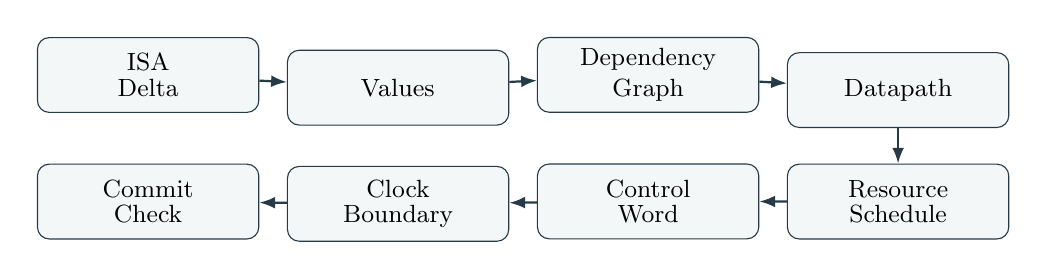
\begin{tikzpicture}[node distance=0.5cm]
\matrix[matrix of nodes,column sep=0.35cm,row sep=0.45cm,nodes={co},ampersand replacement=\&] (m) {
\shortstack{ISA\\Delta} \& Values \& \shortstack{Dependency\\Graph} \& Datapath \\
\shortstack{Commit\\Check} \& \shortstack{Clock\\Boundary} \& \shortstack{Control\\Word} \& \shortstack{Resource\\Schedule} \\
};
\draw[flow] (m-1-1) -- (m-1-2);
\draw[flow] (m-1-2) -- (m-1-3);
\draw[flow] (m-1-3) -- (m-1-4);
\draw[flow] (m-1-4) -- (m-2-4);
\draw[flow] (m-2-4) -- (m-2-3);
\draw[flow] (m-2-3) -- (m-2-2);
\draw[flow] (m-2-2) -- (m-2-1);
\end{tikzpicture}
\end{center}

\subsection*{六个重建问题}
\begin{enumerate}
  \item 指令允许哪些架构状态改变，哪些绝不能改变？
  \item 每个所需值在哪里产生，又在哪里被消费？
  \item 现有通路缺的是路线、选择器、端口还是功能部件？
  \item 哪些动作因依赖、资源或关键路径必须拆拍？
  \item 当前阶段应打开哪些 Enable、Select 和 Command？
  \item 值何时产生、何时可达、何时才真正提交？
\end{enumerate}

\begin{methodbox}{来源处置}
本册吸收了旧笔记中“从功能到数据流、微操作和控制信号”“单总线唯一驱动”“单周期空间换时间、多周期时间换空间”“控制器统一映射”和 LOAD 教学机轨迹。固定九节拍只作为带假设的母例；多核/Flynn、Cache、虚拟存储、完整 I/O、中断软件处理和 ABI 分别交给其 Owner。来源中的绝对 RISC/CISC 对应、通用寄存器可见性清单和特定存储实现结论未进入稳定模型。
\end{methodbox}

\end{document}
